\section{The Higgs Boson}

The Higgs boson is the only scalar particle present in the current formulation
of the SM. It is predicted to be massive with neither electric nor colour
charge. It couples to all massive particles, including itself, with coupling
strengths related to the mass of the particle. The coupling strength of the
Higgs boson to gauge bosons, $V$, is proportional to $m_{V}^2$. Similarly, the
Yukawa interactions between Higgs bosons and fermions are predicted to occur
with strengths proportional to the mass of the fermions, $m_f$. The detection of
the Higgs boson and confirmation of its properties (e.g.\ spin, intrinsic
parity, mass-dependent coupling strengths\todo{CP?}) would represent evidence
for the BEH mechanism and the Glashow--Salam--Weinberg model of the electroweak
interaction.

In 2012, almost half a century after the proposal of the
Glashow--Salam--Weinberg model, the Higgs boson was discovered by the
ATLAS~\cite{HIGG-2012-27} and CMS~\cite{CMS-HIG-12-028} collaborations at the
Large Hadron Collider with a mass of about \SI{125}{\GeV}. Since its discovery,
extensive measurements of its properties have been performed showing remarkable
agreement with the SM predictions. In 2022, the Higgs boson mass has been
measured with relative errors approaching \SI{0.1}{\percent}. An exemplary
measurement of the Higgs boson mass by the ATLAS collaboration yields
\begin{align*}
  m_{H} = \num{124.99}%
  \valuesep\numerrt{0.18}{stat.}%
  \valuesep\numerrt{0.04}{syst.}%
  \valuesep\si{\GeV}
\end{align*}
in the $H \to Z Z^{*} \to 4\ell$ channel~\cite{HIGG-2020-07} using \pp-collision
events collected during Run~2 of the Large Hadron Collider. The scalar nature of
the Higgs boson has been
confirmed~\cite{HIGG-2013-17-witherratum,CMS-HIG-14-018} and its coupling
strengths are thus far in good agreement with the SM
predictions~\cite{HIGG-2021-23,CMS-HIG-22-001}. As a result, the electroweak
sector is well established and the two parameters of the BEH potential, $v$ and
$m_{H}$, are measured with high precision.\footnote{The VEV was known prior to
  the discovery of the Higgs boson through measurements of the muon lifetime
  which allows to determine the effective coupling constant $G_{\text{F}}$ of
  the charged-current weak interaction. With known $G_{\text{F}}$, the VEV can
  be determined according to
  $v = \bigl( \sqrt{2} G_{\text{F}} \bigr)^{-1/2} \approx
  \SI{246}{\GeV}$~\cite{MuLan:2010shf}.}


\subsection{Production and Decay Modes}

The production of Higgs bosons at the LHC occur through different production
modes with production cross sections spanning multiple orders of magnitude. The
Feynman diagrams of the four dominant production modes are shown in
\Cref{fig:higgs_prod_feyn}, all of which have been experimentally confirmed. The
production cross section in \pp-collisions at a centre-of-mass energy of
\SI{13}{\TeV} is shown in \Cref{fig:higgs_prod_xsec} as a function of
$m_{H}$. For $m_{H} = \SI{125.0}{\GeV}$, the \ggF production mode has the
largest production cross section with
$\sigma(\pp \to H) \approx \SI{50}{\pico\barn}$, followed by the the VBF mode
with $\sigma(\pp \to qqH) \approx \SI{4}{\pico\barn}$, the $VH$ mode with
$\sigma(\pp \to VH) \approx \SI{2}{\pico\barn}$ inclusive in $V = W^\pm$ and
$V= Z$, and finally the $\ttbar H$ mode with
$\sigma(\pp \to \ttbar H) \approx
\SI{0.5}{\pico\barn}$~\cite{deFlorian:2016spz}.\todo{The $\ttbar H$ production
  mode allows to access the top Yukawa coupling} Higgs boson production modes
involving two Higgs bosons in the final state, which are the processes of
primary interest for this thesis, are covered in
\Cref{fig:theory_higgs_pair_prod}.

\begin{figure}[htbp]
  \centering

  \begin{subfigure}{0.48\textwidth}
    \centering
    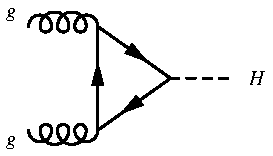
\includegraphics[scale=1]{feynman_graphs/higgs_prod_ggf}
    \subcaption{Gluon-gluon fusion (\ggF)}
  \end{subfigure}%
  \begin{subfigure}{0.48\textwidth}
    \centering
    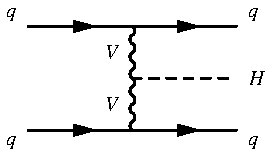
\includegraphics[scale=1]{feynman_graphs/higgs_prod_vbf}
    \subcaption{Vector boson fusion (VBF)}
  \end{subfigure}

  \vspace*{0.5em}

  \begin{subfigure}{0.48\textwidth}
    \centering
    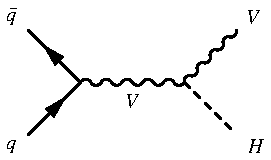
\includegraphics[scale=1]{feynman_graphs/higgs_prod_vh}
    \subcaption{Associated production with a massive vector boson ($VH$)}
  \end{subfigure}%
  \begin{subfigure}{0.48\textwidth}
    \centering
    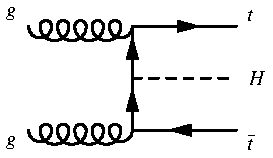
\includegraphics[scale=1]{feynman_graphs/higgs_prod_tth}
    \subcaption{Associated production with \ttbar ($\ttbar H$)}
  \end{subfigure}%

  \caption{The dominant Higgs boson production modes in \pp-collisions at
    centre-of-mass energies of \SI{13}{\TeV}.}%
  \label{fig:higgs_prod_feyn}
\end{figure}

\begin{figure}[htbp]
  \centering

  \begin{subfigure}[b]{0.47\textwidth}
    \centering

    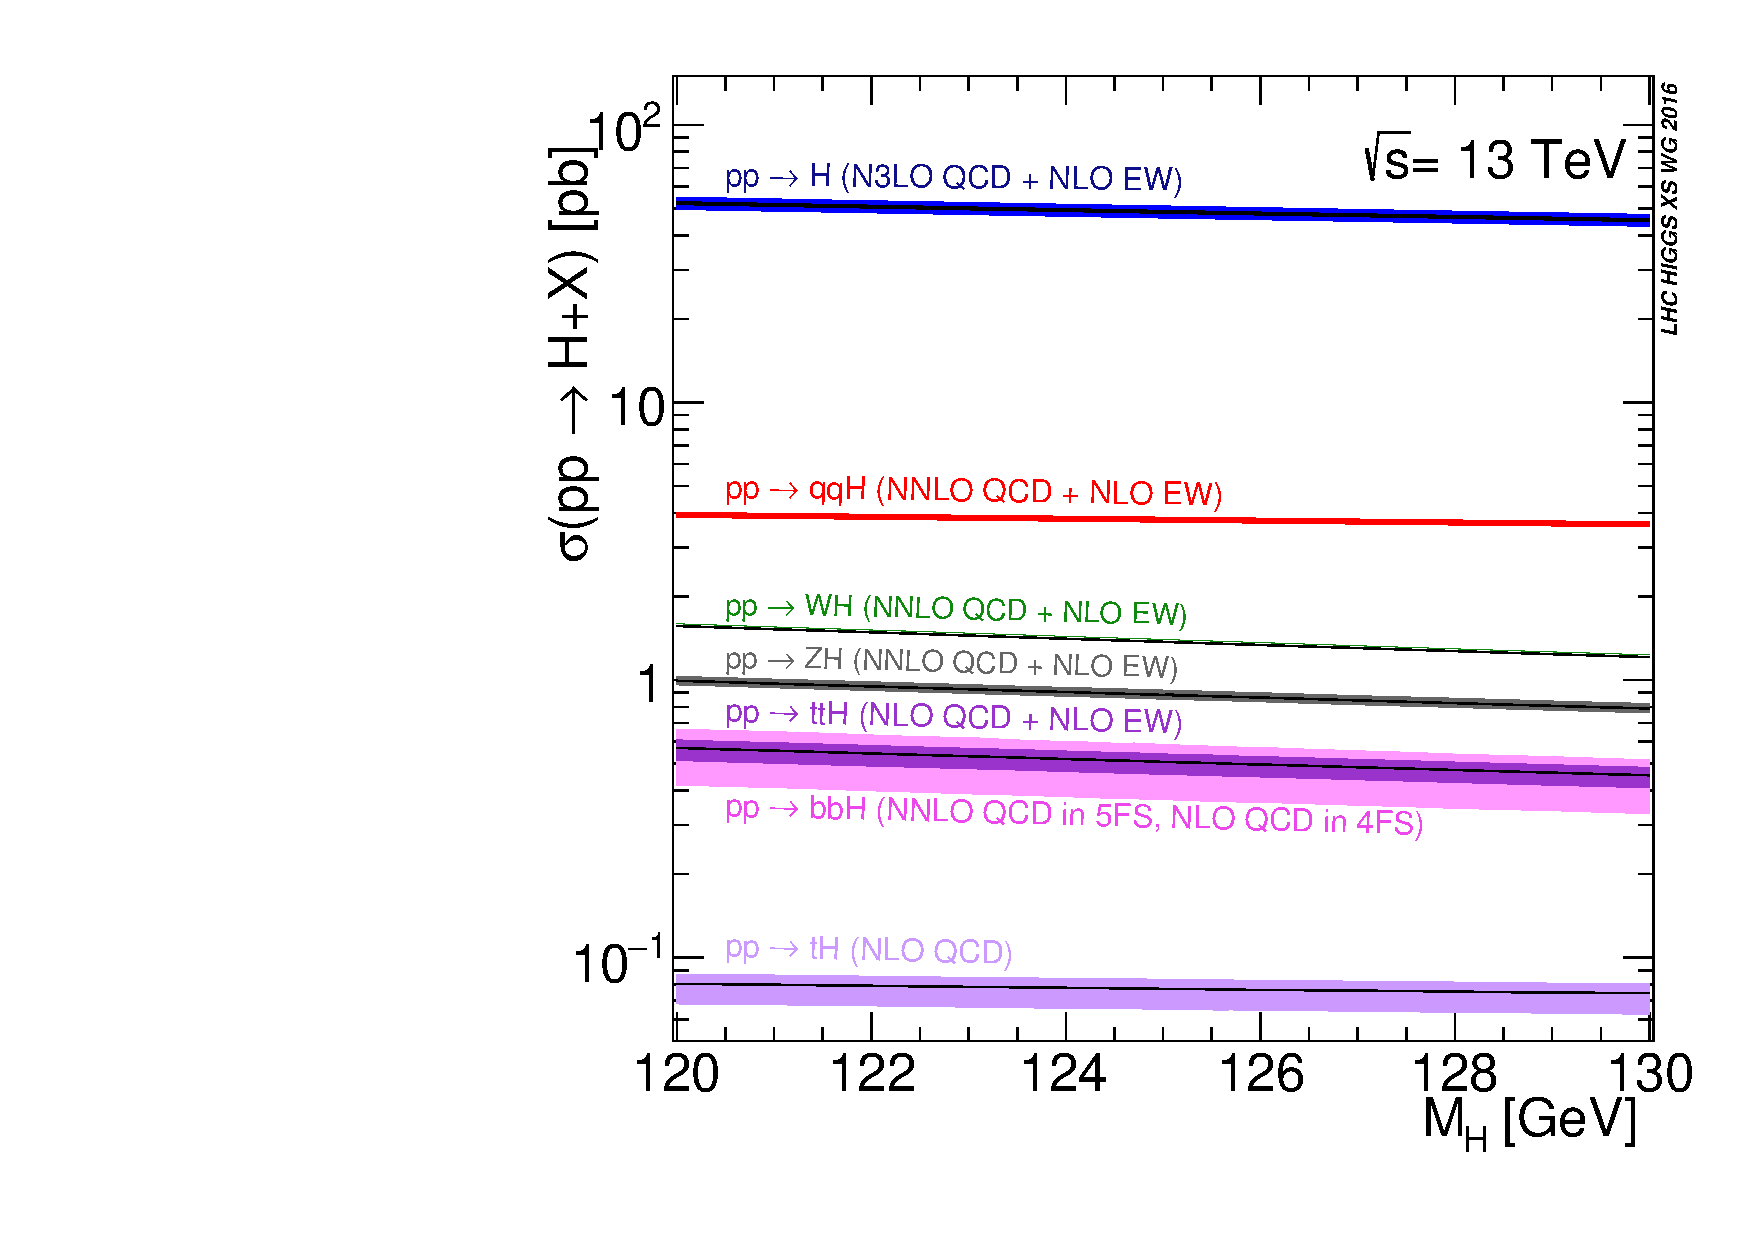
\includegraphics[width=0.95\textwidth]{theory/h_prod_crossec_13tev}

    \subcaption{Cross sections of Higgs boson production modes as a function of
      $m_{H}$.}%
    \label{fig:higgs_prod_xsec}
  \end{subfigure}\hfill%
  \begin{subfigure}[b]{0.47\textwidth}
    \centering

    \renewcommand{\arraystretch}{1.1}%
    \begin{tabular}{lS[table-format=2.3]c}
  \toprule
  Decay mode  & {BR / \%} & Observed \\
  \midrule
  $\bbbar$        & 58    & \checkmark \\
  $W^{+} W^{-}$    & 21    & \checkmark \\
  $gg$            & 8.2   & \\
  $\tau^+ \tau^-$ & 6.3   & \checkmark \\
  $c\bar{c}$      & 2.9   & \\
  $ZZ^{*}$            & 2.6   & \checkmark \\
  $\gamma\gamma$  & 0.23  & \checkmark \\
  $Z\gamma$       & 0.15  & \\
  $\mu^{+}\mu^{-}$ & 0.022 & $\sim$~\cite{CMS-HIG-19-006} \\
  \bottomrule
\end{tabular}

%%% Local Variables:
%%% mode: latex
%%% TeX-master: "../phd_thesis"
%%% End:


    \vspace*{1.2em}

    \subcaption{Branching ratios of Higgs boson decay modes. The $gg$,
      $\gamma\gamma$, and $Z\gamma$ decay modes occur via higher-order
      processes.}%
    \label{tab:higgs_branching_ratios}
  \end{subfigure}

  \caption{Higgs boson production cross section in \pp-collisions at a
    centre-of-mass energy of \SI{13}{\TeV} (a) and Higgs boson decay branching
    ratios for $m_{H} = \SI{125.0}{\GeV}$ (b). The figure and branching ratios
    are taken from Ref.~\cite{deFlorian:2016spz}.}
\end{figure}

The Higgs boson ($m_{H} = \SI{125}{\GeV}$) is predicted to have a total decay
width of about \SI{4}{\MeV}~\cite{deFlorian:2016spz} yielding a proper lifetime
of $10^{-22}\,\si{\second}$. As a result, the Higgs boson decays almost
immediately via one of the decay modes summarised in
\Cref{tab:higgs_branching_ratios} allowing detection only via its decay
products. The table reflects the preferential coupling of the Higgs boson to
heavy particles such as the weak gauge bosons\footnote{The decays of Higgs
  bosons to $W^+W^-$ and $ZZ$ are suppressed since $m_{H} < 2 m_{W} < 2 m_{Z}$
  such that one of the gauge bosons has to be produced \emph{off-shell}.} and
third generation fermions. The vast majority of Higgs bosons decay into \bbbar
with a branching ratio of \SI{58}{\percent}. The $b$-quark is the heaviest
fermion that can be produced in decays of Higgs bosons with
$m_H = \SI{125}{\GeV}$, decays to top-quark pairs being forbidden due to
$m_t > m_H$. The second largest branching ratio to fermions is the decay
$H \to \tau^+ \tau^-$ with \SI{6.3}{\percent} due to the large mass of the
\taulepton of \SI{1.777}{\GeV}~\cite{pdg2020}. In addition, a first indication
of SM-like Yukawa coupling to fermions of the second generation exist in the
form of evidence for the process $H \to \mu^+ \mu^-$ by the CMS
collaboration~\cite{CMS-HIG-19-006}.


\subsection{Higgs Boson Pair Production}%
\label{fig:theory_higgs_pair_prod}

% Super excellent talk by Katharine:
% https://indico.cern.ch/event/1065153/attachments/2351166/4011032/Seminar.pdf

After the discovery of the Higgs boson and the measurement of its mass, the free
parameters of the EWSB in the SM, $v$ and $m_H$, are fully determined and thus
also the form of the BEH potential. An important test of the SM is the
measurement of processes involving the Higgs boson self-coupling. These
processes allow for a direct determination of the cubic and quartic terms in the
BEH potential of \Cref{eq:beh_potential}, thus providing additional checks of
the internal consistency of the SM. The direct measurement of the trilinear and
quartic Higgs boson self-coupling can be performed in final states with two or
three Higgs bosons, respectively. Currently, the direct measurement of the
quartic Higgs boson self-coupling is experimentally infeasible due to the small
cross section of triple Higgs boson production (about \SI{80}{\atto\barn} in
\pp-collisions at $\sqrt{s} = \SI{13}{\TeV}$~\cite{Maltoni:2014eza}). Instead,
the focus of this thesis lies on directly probing the trilinear Higgs boson
self-coupling, $\lambda_{HHH}$, in Higgs boson pair production.\footnote{The
  Higgs boson self-coupling can also be probed indirectly through higher-order
  corrections to the production of single Higgs bosons. See for example
  Ref.~\cite{Degrassi:2016wml} \cite{ATLAS-CONF-2022-050}.}


% Mention this somewhere?
% \lambda &\approx 0.13 \quad \text{(SM)}

The production of Higgs boson pairs at the LHC is a rare process with cross
sections more than 1000 times smaller than the production of single Higgs
bosons. Under the SM hypothesis, Higgs boson pair production is not yet
accessible using data collected during Run~2 of the LHC. However, first evidence
of Higgs boson pair production could be obtained by the end of the LHC
programme. Nevertheless, probing Higgs boson pair production is valuable
already. First, experimental methods can be developed and improved that might
culminate in a discovery towards the end of the LHC programme. Second, possible
deviations from the SM can manifest as enhancements of Higgs boson pair
production to which sensitivity might already exist.


\subsubsection{Production Modes}%

In the SM, Higgs boson pairs are produced non-resonantly yielding final states
with two real (on-shell) Higgs bosons. Several production modes of Higgs boson
pairs are predicted by the SM. The following description assumes \pp-collisions
at $\sqrt{s} = \SI{13}{\TeV}$ and $m_{H} = \SI{125.0}{\GeV}$.

The gluon-gluon fusion process (\ggF) is the dominant production mode of Higgs
boson pairs in the SM (SM $HH$). The leading order diagrams of this process are
depicted in \Cref{fig:dihiggs_ggf_feyn}. Both diagrams involve a loop of heavy
quarks, the loop being dominated by top-quarks due to their large coupling to
the Higgs boson. The box diagram depicted in \Cref{fig:dihiggs_ggf_feyn_box}
does not involve any Higgs boson self-interaction vertices.\footnote{As a
  result, Higgs boson pair production exists even in the absence of Higgs boson
  self-interactions.} However, the triangle diagram in
\Cref{fig:dihiggs_ggf_feyn_triangle} does involve the Higgs boson self-coupling
thus making SM $HH$ production sensitive to $\lambda_{HHH}$. The triangle and
the box diagram interfere destructively leading to a small SM $HH$ production
cross section via \ggF of
\begin{align*}
  \sigma(pp \to HH) = \SI{31.05}{\femto\barn}
\end{align*}
at NNLO~\FTapprox~\cite{Grazzini:2018bsd}.

\begin{figure}[htbp]
  \centering

  \begin{subfigure}{0.49\textwidth}
    \centering
    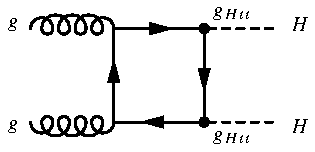
\includegraphics[width=0.7\textwidth]{feynman_graphs/di_higgs_box}
    \subcaption{}%
    \label{fig:dihiggs_ggf_feyn_box}
  \end{subfigure}\hfill%
  \begin{subfigure}{0.49\textwidth}
    \centering
    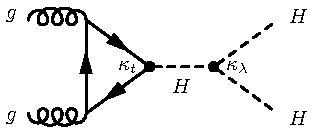
\includegraphics[width=0.7\textwidth]{feynman_graphs/di_higgs_triangle}
    \subcaption{}%
    \label{fig:dihiggs_ggf_feyn_triangle}
  \end{subfigure}

  \caption{Feynman diagrams of Higgs boson pair production via \ggF at leading
    order. The diagrams (a) and (b) are commonly referred to as the box and
    triangle diagrams, respectively. The Higgs boson self-coupling and the
    top-quark Yukawa coupling is indicated by $\lambda_{HHH}$ and $g_{Htt}$,
    respectively.}%
  \label{fig:dihiggs_ggf_feyn}
\end{figure}

The second largest SM \HH production mode is vector boson fusion (VBF). The
leading order diagrams of the VBF production mode are depicted in
\Cref{fig:dihiggs_vbf_feyn}. The diagrams involve the coupling of the Higgs
boson to vector bosons, $g_{HVV}$, the quartic $HHVV$ coupling, $g_{HHVV}$, and
the Higgs boson self-coupling. A characteristic feature of the VBF production
mode is the presence of two additional jets originating from the fragmentation
and hadronisation of the final state quarks. The predicted SM \HH production
cross section via VBF is
\begin{align*}
  \sigma(\pp \to qqHH) = \SI{1.726}{\femto\barn}
\end{align*}
at $\text{N}^3\text{LO}$~\cite{Dreyer:2018qbw,LHCHWGHH}. Due to the small cross
section, the VBF production mode is currently of lesser relevance to probe the
nature of the Higgs boson self-coupling.

\begin{figure}[htbp]
  \centering

  \begin{subfigure}{0.33\textwidth}
    \centering
    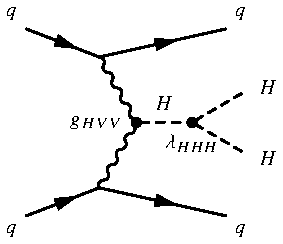
\includegraphics[width=0.95\textwidth]{feynman_graphs/di_higgs_vbf_kvklam}
    \subcaption{}
  \end{subfigure}\hfill%
  \begin{subfigure}{0.33\textwidth}
    \centering
    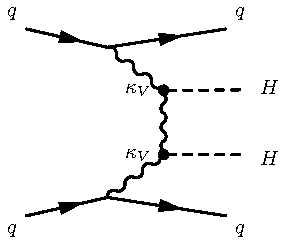
\includegraphics[width=0.95\textwidth]{feynman_graphs/di_higgs_vbf_kvkv}
    \subcaption{}
  \end{subfigure}\hfill%
  \begin{subfigure}{0.33\textwidth}
    \centering
    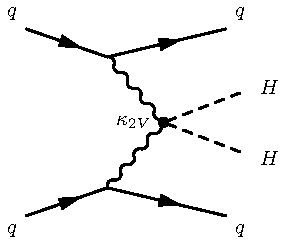
\includegraphics[width=0.95\textwidth]{feynman_graphs/di_higgs_vbf_ktwov}
    \subcaption{}
  \end{subfigure}

  \caption{Feynman diagrams of Higgs boson pair production via VBF at leading
    order.}%
  \label{fig:dihiggs_vbf_feyn}
\end{figure}

Additional production modes of SM \HH with even smaller cross sections
exist. Examples of these are the associated production of \HH with weak vector
bosons with
$\sigma(\pp \to VHH) \approx \SI{0.9}{\femto\barn}$~\cite{deFlorian:2016spz}
($V = W^\pm\,\text{or}\,Z$) and associated production with \ttbar with
$\sigma(\pp \to \ttbar HH) \approx
\SI{0.8}{\femto\barn}$~\cite{deFlorian:2016spz}. These production modes are not
considered in the remainder of this thesis.


\subsubsection{Decay Channels of Pairs of SM Higgs Bosons}%

With the observed mass of the Higgs boson of about \SI{125}{\GeV}, a large
number of Higgs boson decay modes are of experimental interest to probe the
nature of the EWSB in the SM. When considering decays of Higgs boson pairs, this
results in a plethora of final states with often distinct signatures.  An
overview of the branching ratios of a system of SM Higgs boson pairs is given in
\Cref{fig:hh_branching_ratios}.

\begin{figure}[htbp]
  \centering

  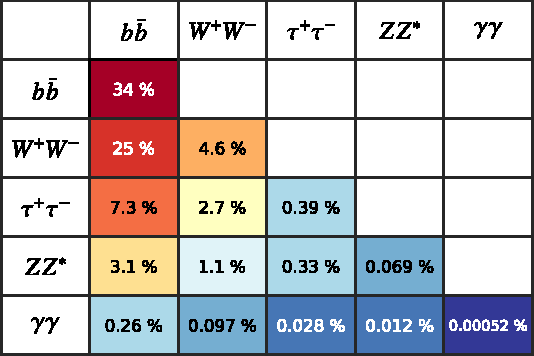
\includegraphics[width=0.5\textwidth]{theory/di_higgs_branching_ratio}

  \caption{Possible final states of decays of pairs of Standard Model Higgs
    bosons. Higgs boson branching ratios are taken from
    Ref.~\cite{deFlorian:2016spz} and assume~$m_{H} = \SI{125.0}{\GeV}$. The
    decay mode~$H \ra g g$ is excluded due to limited experimental feasibility.}%
  \label{fig:hh_branching_ratios}
\end{figure}

Experimentally, searches for SM \HH production have to make a compromise between
the branching ratio of the decay channel, the ability to select the relevant SM
\HH events, and the background contributions from other processes. Currently,
the most sensitive search channels for SM \HH production are:
\begin{description}

\item[The \bbbb channel] has the largest branching ratio (\SI{34}{\percent}) of
  any final state resulting from the decay of a Higgs boson pair. However, this
  channel is dominated by backgrounds from QCD multi-jet production due to its
  fully hadronic final state. As a result, selecting signal events is
  challenging and requires $b$-jet triggers with strict transverse momentum
  thresholds.
  % Moreover, identifying the individual $H \to \bbbar$ candidates
  % -> Not a huge problem for SM

\item[The \bbtautau channel] has a reduced branching ratio (\SI{7.3}{\percent}),
  however, the presence of two \tauleptons provides a decent signature to select
  signal events and suppression of the QCD multi-jet background. In addition,
  relevant backgrounds in this channel are the production of \ttbar, \Zjets, and
  single Higgs bosons. Searches for SM \HH in the \bbtautau channel often focus
  on final states with one leptonic and one hadronic \taulepton decay (\lephad),
  and final states with two hadronic taulepton decays (\hadhad). These final
  states cover almost \SI{90}{\percent} of $HH \to \bbtautau$ events.

\item[The \bbyy channel] has a very small branching ratio (\SI{0.26}{\percent})
  but the photon pair provides an outstanding signature to select signal
  events. Additionally, the reconstruction of the di-photon invariant mass,
  $m_{\gamma\gamma}$, has a typical resolution of \SIrange{1}{2}{\GeV} in the
  ATLAS and CMS experiments at the
  LHC~\cite{PERF-2007-01,CMS-CMS-00-001}.\footnote{Compared to the typical
    resolutions of $H \to \bbbar$ and $H \to \tautau$ reconstruction in the
    \bbbb and \bbtautau channels, this represents an improvement of about an
    order of magnitude.} Therefore, $m_{\gamma\gamma}$ provides an excellent
  discriminant to reject most background processes leaving only continuum
  $\gamma\gamma$ and single Higgs boson production as relevant background
  processes.

\end{description}


\subsubsection{Experimental Status}%

The experimental status prior to the work of this thesis.

Comparisons of the results obtained in this thesis with the latest ones are
given in the respective subchapters.





\clearpage
\todo[inline]{Here be dragons}


\begin{description}

\item[Vacuum Stability] The present minimum with a vacuum expectation
  value of $v \approx \si{246}{\GeV}$ might be either a global minimum
  in which case the universe is stable or only a local minimum which
  leads to a metastable universe. In the metastable case, the state of
  the Higgs field could tunnel to a new local or global minimum with a
  smaller vacuum expectation value. Current experimental data cannot
  distinguish whether the universe is stable or
  meta-stable\todo{citation}.

\item[Elektroweak phase transition] In baryogenesis a first order
  electroweak phase transition is needed.

\item[BSM] Radions, 2HDM, Warped extra dimensions, composite Higgs, hMSSM, KK
  Gravitons: Most could decay to pairs of SM Higgs bosons.

\end{description}

\todo[inline]{Shortcomings of the SM: Hierarchy problem, dark matter, quantum
  description of gravity}

\todo[inline]{Maybe: SUSY - superpartners - cancellation of loop corrections to $h$
  mass; In R-parity conserving SUSY - LSP - DM candidate}

\todo[inline]{What models predict Spin-0 resonances decaying into pair of SM
  Higgs? 2HDM}

\todo[inline]{Mention Spin-2 resonances? KK-graviton -- theoretically not favoured}

\todo[inline]{Scalar sector relatively unexplored?}

%%% Local Variables:
%%% mode: latex
%%% TeX-master: "../../phd_thesis"
%%% End:
